\chapter{TrackCIS, un outil au service de l'interopérabilité des applications
hospitalières}
	\paragraph{}
	Cette première grande partie est une introduction du projet sur lequel porte ce
	mémoire. Ce projet s'inscrit dans des enjeux propres à la société Xperis et
	porte sur l'outil TrackCIS, console de supervision de l'EAI Cloverleaf. Tous
	ces termes pouvant paraître un peu flous, nous nous attacherons ici à présenter
	les différents éléments importants de notre étude de façon à en cerner tous
	les enjeux et à mettre en place une méthodologie adaptée.

	\subsection{TrackCIS est une console de supervision de l'EAI Cloverleaf}
		\paragraph{}
		Commençons par définir quelques notions techniques qui nous seront utiles,
		sinon indispensables pour la suite : les EAI et leurs consoles de supervision.
		
		\subsubsection{Qu'est-ce qu'un EAI ?}
			\paragraph{}% Interopérabilité
			EAI signifie Intégration d'Applications d'Entreprise. Pour bien comprendre de
			quoi il s'agit et quel rôle tient un tel outil dans un système d'information
			(SI), il nous faut comprendre la notion d'interopérabilité. Il est important
			de préciser que nous ne parlerons dans cette partie - et plus généralement
			tout au long de ce document - que des EAI dans le monde hospitalier. En
			effet, de nombreuses entreprises ou organismes de tous les secteurs utilisent
			de tels outils. Dans notre cas nous nous focaliserons uniquement sur les EAI du
			monde hospitalier et nous chercherons à comprendre ce que sont les EAI au
			travers d'exemples de ce secteur.\newline
			Selon la définition du dictionnaire Larousse, l'interopérabilité est la
			"capacité de matériels, de logiciels ou de protocoles différents à
			fonctionner ensemble et à partager des informations"
			\citep{larousse_definitions_interop}. Si l'on transpose cette définition au
			monde de l'hôpital, l'interopérabilité correspond à la capacité des
			différents logiciels (ou applicatifs) métier à fonctionner ensemble. Il
			existe une grande diversité d'applicatifs métier dans ce secteur. Le
			\ref{exemple_appli} offre un aperçu de quelques fonctions
			remplies par les logiciels que l'on peut trouver dans un hôpital.
			\begin{table}[H]
				\centering
				\begin{tabular}{| p{4cm} | p{10cm} |} %Exemples des principaux logiciels
				% métier
					\hline
					\thead{Type de fonctionnalité}&\thead{Description}
					\\
					\hline
					La GAM (Gestion Administrative des Malades)
					&
					Bla bla bla bla
					\\
					\hline
					Le DPI (Dossier Patient Informatisé)
					&
					Le DPI 
					DPI et GAM sont les deux princpaux outils utilisés dans les centres
					hospitéliers. De nombreux éditeurs proposent des logiciels permettant de
					remplir ces fonctions.\\
					\hline
				\end{tabular}
				\caption{\label{exemple_appli}Quelques fonctions assurées par les
				logiciels métiers présents dans les hôpitaux
				\citep{interopsante_guide_2015}.}
			\end{table}
			Or ces différents outils ont bien souvent été développés par des sociétés
			différentes. En outre, chacun est spécialisé dans quelques fonctions
			bien précises : comptabilité, enregistrement des patients, gestion des
			stocks de pharmacie\ldots Dans la plupart des cas, leur conception ne leur
			permet pas de fonctionner ensemble, ce qui pourtant peut s'avérer utile. Par
			exemple, le logiciel gérant les stocks de la pharmacie peut avoir besoin
			d'informations sur les prescriptions faites par les médecins aux patients. De
			même, les données sur les patients saisies à l'arrivée de ces derniers
			peuvent intéresser les médecins dans le logiciel gérant les dossiers
			médicaux. En résumé, il est nécessaire pour ces différentes applications de
			partager des données les unes avec les autres.
			
			\paragraph{}% L'EAI est la solution au problème de l'interopérabilité
			C'est ici qu'entre en jeu l'EAI. Il s'agit d'un outil capable d'établir des
			connexions entre les applications métier. Il va par exemple collecter
			certaines données émises par le logiciel de gestion des entrées patients
			pour les injecter dans l'outil de gestion des dossiers médicaux. Plus
			généralement, il transfert des données émises par un outil A pour les
			mettre à disposition d'un outil (figure \ref{intro_interop}).
			\begin{figure}[H]
				\centering
				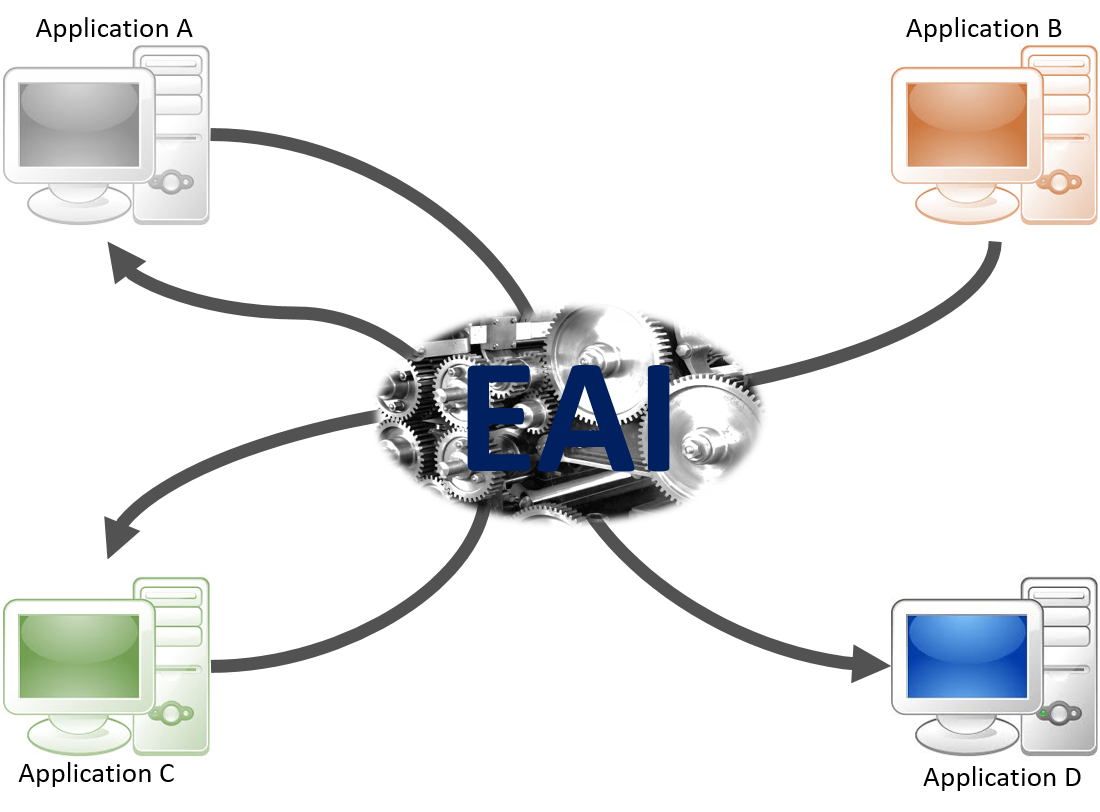
\includegraphics[width=10cm]{../img/eai_1.png}
				\caption{\label{intro_interop} L'EAI est un outil qui permet
				d'établir des routes entre applications métier.}
			\end{figure}
			Cloverleaf est un EAI dédié au monde hospitalier (il n'est cependant pas le
			seul).
			
			\paragraph{}% transfo de messages
			Les fonctions de l'EAI ne se résument pas au seul transport des données. Il
			est parfois utile de réaliser des actions sur les informations transmises
			d'une application à l'autre (figure \ref{interop_transfo}). Ces actions
			peuvent êtres par exemple :\newline
			\begin{itemize}
			  \item de valider les informations transmises. Par exemple, l'EAI va
			  s'assurer que pour chaque donnée émise par une application de gestion des
			  prescriptions, le nom du patient est bien présent.
			  \item d'effectuer des transformations. L'application destinataire ne
			  gère pas forcément les mêmes formats de données que l'application émettrice
			  car, rappelons-le, les applications ne sont pas forcément conçues pour
			  fonctionner ensemble. L'EAI est ainsi capable de faire des conversions de
			  format de donnée.\newline
			\end{itemize}
			\begin{figure}[H]
				\centering
				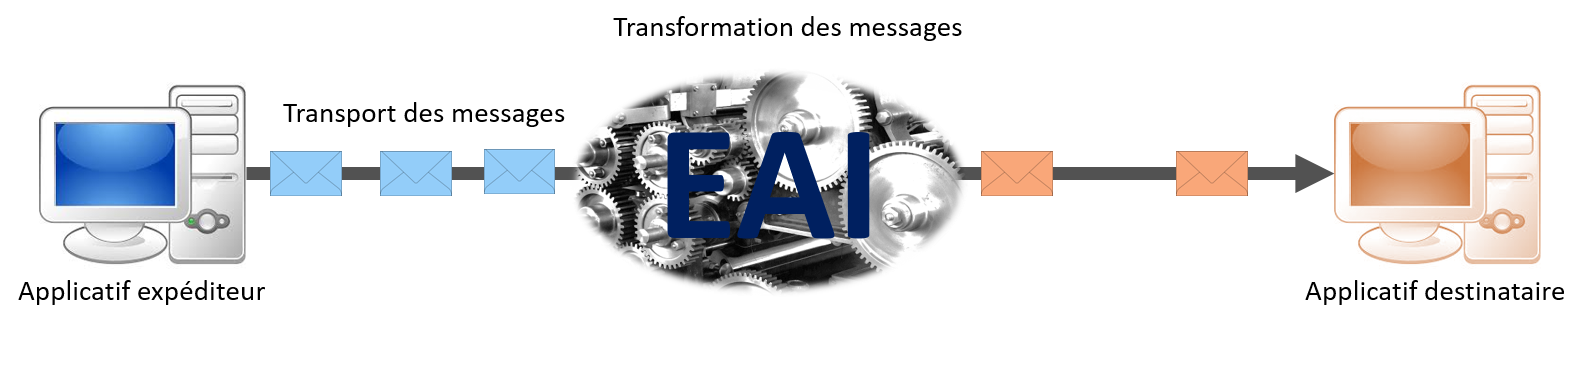
\includegraphics[width=15cm]{../img/eai_2.png}
				\caption{\label{interop_transfo} Un EAI peut effectuer des opérations sur
				les données qui transitent par lui.}
			\end{figure}
			
			\paragraph{}% Un peu de vocabulaire
 			Il existe un vocabulaire pour désigner les transferts de données entre
 			applications. Dans la suite, nous parlerons de :
 			\begin{description}
 				\item[Flux] Les flux sont tout simplement les routes permettant de
 				connecter une application à une autre. Dans un système d'information hospitalier
 				(SIH), il y a donc autant de flux que de couple d'application. Il est
 				possible - et même courant - qu'une application soit reliée à plusieurs
 				autres.
 				\item[Message] Les données qui passent le long des flux, d'une application
 				à une autre, sont appelées messages. Les messages se présentent en général
 				sous la forme de texte hautement standardisé. Les messages sont émis par les
 				applicatifs métier dans un format donné. Il existe de nombreux formats
 				dont certains sont spécifiques au monde hospitalier. L'annexe 1 présente
 				quelques-uns des principaux formats utilisés (les formats HL7 et HPRIM).
 			\end{description}

		\subsubsection{Les flux de messages doivent être surveillés}
			\paragraph{}% Importance fonctionnelle de la supervision
			L'EAI est un outil complexe et dont le bon fonctionnement est essentiel. En
			effet, c'est tout le SI de l'hôpital qui repose en permanence sur lui. Si
			un disfonctionnement intervient, des pans entiers du
			service hospitalier risquent d'en pâtir, ce qui aura des conséquences sur le
			traitement des patients. Lorsqu'un disfonctionnement survient au niveau d'un
			flux, au point que celui-ci ne peut plus transmettre ses messages, on dit
			qu'il tombe en erreur.

			\paragraph{}% Exemple de cas de disfonctionnement
			Il existe différentes raisons pour lesquelles un flux peut tomber en erreur.
			La figure \ref{interop_erreur} expose les trois principales. La cause (1)
			évoquée sur le schéma, correspond à une erreur qui survient entre l'application source et l'EAI,
			c'est-à-dire lors du transfert du message de l'application à l'EAI. Une
			erreur de ce type peut avoir des causes variées. Il peut s'agir d'un problème
			au niveau du réseau qui transporte les messages (par exemple une coupure
			d'internet). Le cas (2) correspond à une erreur qui est levée
			lors du traitement du message par l'EAI. Il se peut que le contenu du
			message ne soit pas conforme à ce qu'attendait le script réalisant le
			traitement. Ce peut être par exemple le cas lorsqu'un utilisateur de
			logiciel métier fait un erreur de saisie et que cette erreur n'est pas
			relevée par le logiciel en question. Enfin, dans le cas (3), les messages
			s'accumulent à la sortie de l'EAI car la route entre l'EAI et l'application
			destinataire est bloquée, par exemple par une coupure momentanée du réseau.
			\newline
			\begin{figure}[H]
				\centering
				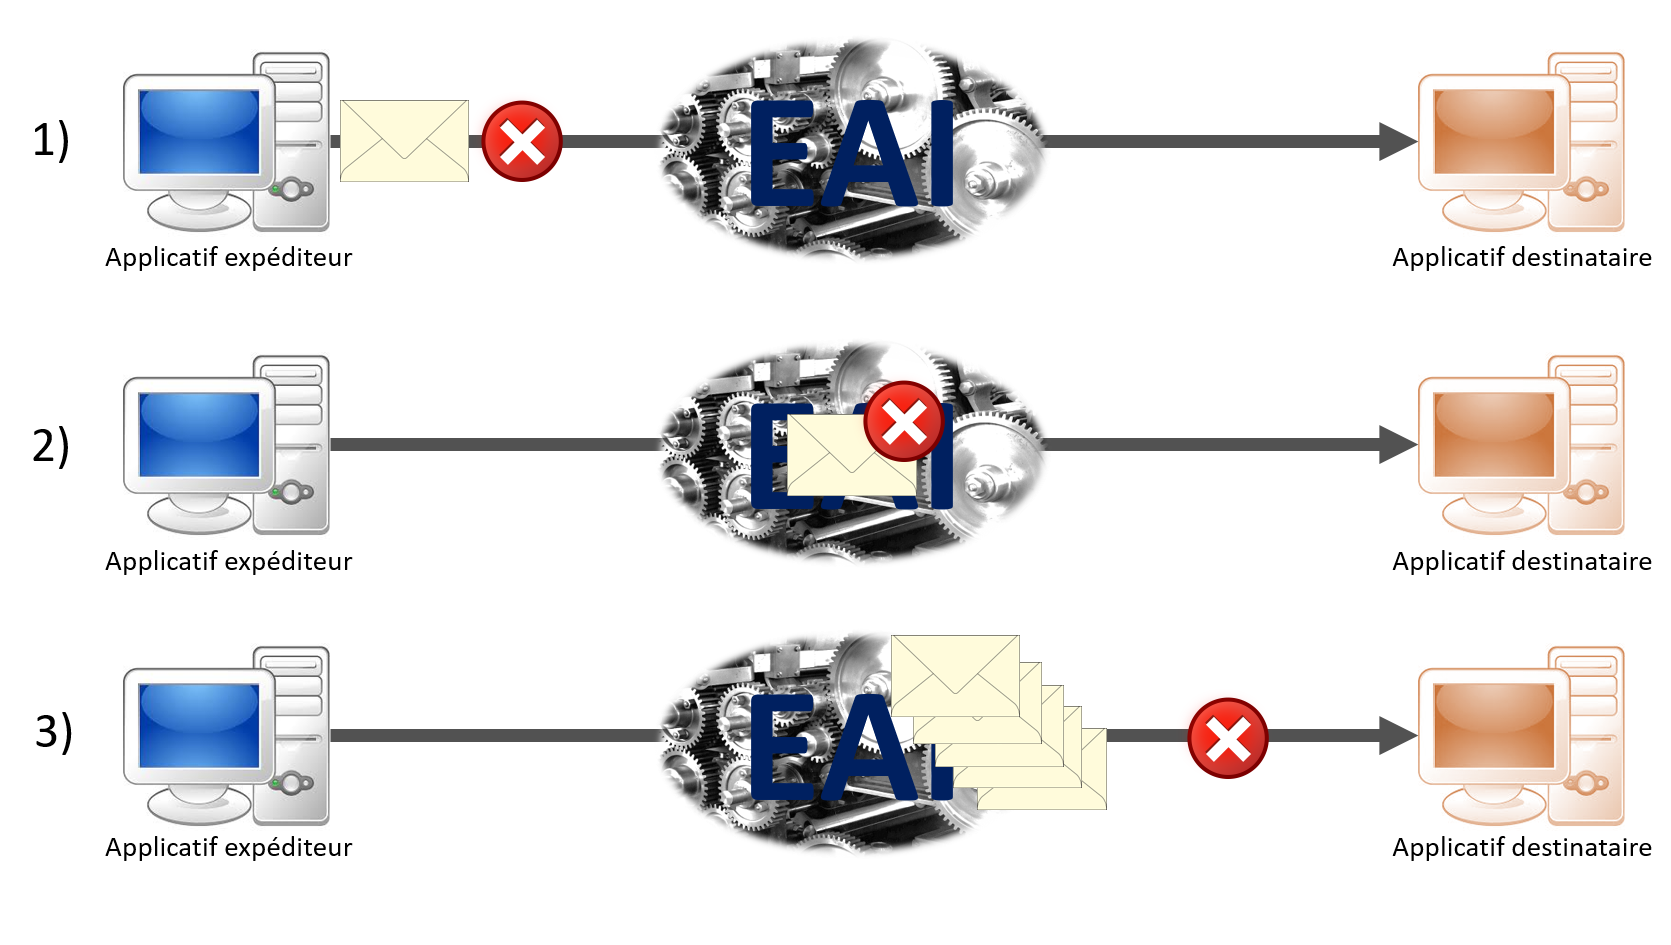
\includegraphics[width=15cm]{../img/error_1.png}
				\caption{\label{interop_erreur} De multiples causes d'erreurs peuvent
				stopper momentanément un flux de message.}
			\end{figure}
			
			\paragraph{}% Surveiller un flux c'est pas facile
			Ainsi, il est capital d'exercer une surveillance continue sur les différents
			flux, pour être certain que l'EAI assure bien ses fonctions et que les
			messages transitent correctement. Cette surveillance est ce que l'on appelle
			la supervision des flux. Cette tâche peut être assurée grâce à deux outils :
			\begin{itemize}
			  \item L'environnement de développement intégré (IDE) de Cloverleaf. Cet
			  outil permet de contrôler tout l'EAI, c'est-à-dire aussi bien assurer la
			  supervision que de mettre en place de nouveaux flux. L'IDE est un outil
			  très complexe qui nécessite une formation spécialisée, ce que les
			  personnels des services informatiques des centres hospitaliers n'ont pas
			  forcément.
			  \item Les consoles de supervision.
			\end{itemize}
			
		\subsubsection{TrackCIS est un outil qui permet la supervision des flux}
			\paragraph{}% C'est quoi une console de supervision ?
			Une console de supervision permet d'assurer la surveillance
			de tout ou partie des flux gérés par l'EAI. Elle dispose d'un
			nombre limité de fonctionnalité par rapport à l'IDE mais se veut plus simple
			et plus rapide d'utilisation. Il existe actuellement pour Cloverleaf un
			certain nombre de consoles :
			\begin{description}
				\item[Global Monitor] Cette console est développée par le même éditeur qui
				est à l'origine de Cloverleaf : Infor. Global Monitor est un outil assez
				complexe, il est destiné à des personnes relativement rompues au
				fonctionnement de l'EAI.
				\item[EAI Supervision] Cet outil est développé par l'un des plus gros
				éditeurs de logiciels hospitalier français : Maincare. Cette console ne
				permet cependant pas de gérer tous les flux, mais seulement ceux faisant
				intervenir des applications développées par Maincare.
				\item[TrackCIS] Cette console a été développée par Xperis. Elle est destinée
				à des utilisateur ne maîtrisant pas forcément l'EAI.
			\end{description}
			
			\paragraph{}% Les principales fonctionnalités
			Nous nous focaliserons dans la suite sur la console de supervision TrackCIS.
			En voici les principales fonctionnalités :
			\begin{itemize}
			  \item Visualiser la liste des messages qui transitent dans le flux en temps
			  réel. L'utilisateur peut ainsi voir les données qui passent par l'EAI. Il
			  a accès à des informations sur ces messages comme leur date d'émission, ou
			  leur état. Ils peuvent par exemple voire si un message est en erreur, c'est
			  à dire s'il est bloqué quelque part dans l'EAI.
			  \item Pouvoir éditer et rejouer les messages. Lors d'une erreur, il peut
			  être utile pour la personne en charge de la supervision de pouvoir modifier
			  à la main le contenu du message. Ceci peut s'avérer utile quand l'erreur
			  est due à une erreur de saisie par l'utilisateur de l'application de
			  départ.
			  \item La rejoue de message. Une fois une erreur corrigée, l'utilisateur de
			  la console peut rejouer le message, c'est à dire le refaire passer dans
			  l'EAI de façon à ce qu'il rejoigne l'application destinataire. La rejoue de
			  message peut également s'avérer utile lors de problèmes de réseau. Une
			  coupure momentanée du réseau peu bloquer les messages qui transitent à ce
			  moment. Une fois la coupure résolue, il faut rejouer les messages pour les
			  débloquer et les faire transiter correctement.
			\end{itemize}
		
		\paragraph{}% Résumé de la partie 1.1
		Nous avons vu dans cette première partie que l'EAI est une solution au
		problème de l'interopérabilité en établissant des flux de données entre
		applications métier. Nous avons souligné le fait que la surveillance (la
		supervision) continue des flux est indispensable au bon fonctionnement de
		l'EAI et, par extension, de tout le SI. Enfin, TrackCIS est un outil qui
		permet de rendre la supervision plus simple et plus rapide.\newline
		Dans la suite nous découvrirons les problématiques inhérentes à cet outil.
		
	\subsection{TrackCIS est au cœur d'une problématique commerciale pour Xperis}
		\paragraph{}
		Précédemment nous avons établi les bases des problématiques d'interopérabilité
		des établissements hospitaliers. Xperis est une entreprise qui propose
		d'accompagner ces derniers dans la mise en place et le maintien de Cloverleaf.
		
		\subsubsection{Xperis est l'intermédiaire dans la distribution de Cloverleaf}
			\paragraph{Infor :}
			C'est la société américaine qui développe l'EAI Cloverleaf. Infor distribue
			son EAI dans de nombreux pays du monde par l'intermédiaire de sociétés
			telles que Xperis.
			
			\paragraph{Les éditeurs :}
			Les éditeurs de logiciels médicaux sont de grosses sociétés dont la
			croissance est assurée par de nombreuses fusions et acquisitions. Ainsi ils
			proposent des solutions logicielles très diverses, car initialement
			développées par des sociétés différentes. Ce sont ces entreprises qui
			achètent l'EAI et le mettent en place chez leurs clients, les hôpitaux. Parmi
			les principaux éditeurs du monde hospitalier on trouve :
			\begin{itemize}
				\item Maincare
				\item Le SIB (Syndicat Interhospitalier de Bretagne)
				\item Le MIPIH (Midi Picardi Informatique Hospitalière)
			\end{itemize}
			
			\paragraph{Xperis :}
			Xperis est le seul distributeur (ou master distributeur) de la solution
			Cloverleaf en France. La société est basée à Bordeaux, compte une dizaine de
			salariés et est l'intermédiaire entre Infor et les éditeurs.
			Même si ces derniers sont les principaux clients de l'entreprise,
			l'entreprise cherche actuellement à établir des relations commerciales
			directes avec les établissements hospitaliers.\newline
			La figure \ref{xperis_secteur} résume les interactions qui existent entre
			tous ces acteurs.
			\begin{figure}[H]% Position d'Xperis dans le secteur de la santé
				\centering
				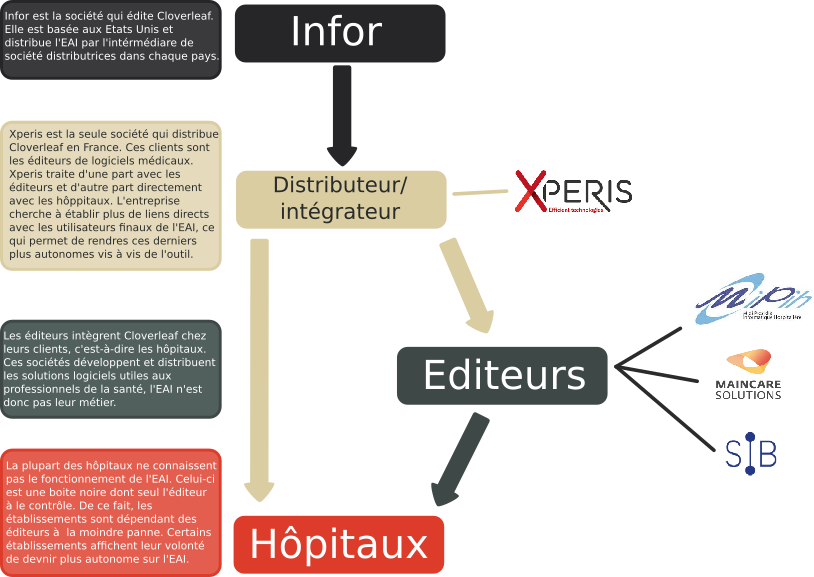
\includegraphics[width=17cm]{../img/xperis_secteur.png}
				\caption{\label{xperis_secteur} Xperis est l'intermédiaire entre Info et
				les éditeurs français.}
			\end{figure}
			
		\subsubsection{Xperis cherche à établir des liens directs avec les hôpitaux}
			\paragraph{}% panorama du monde hospitalier
			Le dernier parti prenant à présenter, qui est l'utilisateur final de
			Cloverleaf, est l'ensemble des établissements hospitaliers français. Au 31
			décembre 2014, on dénombrait en France 3 111 établissements hospitaliers,
			dont 1 416 établissements publics. Ces derniers sont répartis en trois
			catégories \citep{drees_panoramas_2016} :
			\begin{itemize}
				\item 182 centres hospitaliers régionaux (CHR) : ils dispensent des soins 
				spécialisés à la population de la région,
				\item 973 centres hospitaliers (CH) : ils assurent les soins médicaux, 
				chirurgie et prise en charge des personnes âgées,
				\item 97 centres hospitaliers psychiatriques,
				\item 164 établissements de soins longue durée.
			\end{itemize}
			Les hôpitaux privés sont répartis en deux catégories :
			\begin{itemize}
				\item 1 012 établissements privés à but lucratif,
				\item 683 établissements à but non lucratif, dont 21 centre de lutte contre 
				le cancer.
			\end{itemize}
			
			\paragraph{}% regroupement des hôpitaux en GHT
			Depuis 2016, une directive nationale prévoit le regroupement des établissements de 
			santé publics français en groupements hospitaliers de territoire (GHT) 
			\citep{valls_decret_2016}. Dans le cadre d'un GHT, les établissements doivent mettre 
			en commun leur système d'informations et doivent utiliser les mêmes logiciels et 
			applicatifs métiers. Le décret prévoit en outre la création de 135 GHT  
			\citep{touraine_marisol_2016}. Ceci risque d'impacter l'activité d'Xperis dans la 
			mesure où, lorsque les GHT seront formés, les outils d'interopérabilités 
			(les EAI) seront également mutualisés.
			
			\paragraph{}% Maincaire va peut-être se séparer d'Xperis un jour
			Le business-modèle d'Xperis repose sur les problèmes d'interopérabilités des 
			éditeurs. Or certains éditeurs cherchent à résoudre ce problème par
			eux-mêmes. C'est par exemple le cas de Maincare, le plus gros client
			d'Xperis. L'entreprise affiche depuis quelques mois la volonté de développer
			sa propre solution d'interopérabilité \citep{perochon_e-sante:_2016}. Le
			risque pour Xperis est donc, à terme, de perdre son plus important client. 
			
			\paragraph{}% La stratégie d'Xperis face à ces challenges
			Pour préparer cette éventualité, l'entreprise cherche de plus 
			en plus à traiter directement avec les établissements hospitaliers. TrackCIS
			contribue à cela puisqu'il s'agit d'un outil développé en interne et
			distribué directement aux hôpitaux.
			
		\subsubsection{Un outil qui se vend mal et qui est peu utilisé}
			\paragraph{}% L'objectif initial du projet TrackCIS
			Comparativement aux autres consoles de supervision, TrackCIS se veut plus
			simple et plus ergonomique. Initialement, le public visé était les
			utilisateurs métier, c'est-à-dire des personnes ne travaillant pas dans le
			milieu informatique comme par exemple des infirmiers ou des pharmaciens. Ces
			personnes, ou référents métiers, sont des utilisateurs d'applications
			médicales. Le projet de TrackCIS avait pour objectif de confier une partie de
			la supervision de l'EAI à ces personnes, sur les flux qui les intéressaient.
			Ainsi, si un utilisateur rencontre un problème lié à l'interopérabilité avec
			une des applications (par exemple un patient enregistré à l'accueil mais dont
			les informations ne sont pas présentent dans le logiciel de gestion des
			dossiers médicaux), il peut se tourner vers le référent métier plutôt que
			vers le service informatique. Ce type de démarche permettrait de supprimer
			des intermédiaires et donc de diminuer le temps de résolution des problèmes.
			
			\paragraph{}% Le problème actuel avec cet outil
			Mais le projet TrackCIS n'a pas pris et même si quelques consoles ont été
			vendues, peu de CH l'utilise pleinement. Les raisons à cela peuvent être
			multiples et relativement méconnues d'Xperis. L'une d'elles est que la
			console n'est pas vendue pré-paramétrée et que c'est au CH de faire ce
			paramétrage.
			Celui-ci peut représenter une charge assez lourde. Une autre raison serait
			que les référents métiers ne soient pas encore mis en place dans les
			hôpitaux.
			
	% Résumé de la partie 1.2
	\paragraph{}
	Nous avons vu qu'Xperis est confronté à un certain nombre de problématiques
	commerciales. L'entreprise à une vraie volonté de traiter en direct avec les
	hôpitaux pour gagner en indépendance vis à vis des éditeurs. TrackCIS entre
	dans cette stratégie mais a du mal à se faire une place parmi les
	clients.\newline
	L'ensemble de ces problématiques constitue le socle de notre travail.
	
	\subsection{Vers une nouvelle version de TrackCIS}
		\paragraph{}% problème => solution commerciale ou solution fonctionnelle
		Le problème que pose TrackCIS soulève une question : pourquoi cet outil ne se
		vend-il pas ? La réponse à cette question, loin d'être triviale, pourrait
		être de deux natures: une solution commerciale et une solution fonctionnelle.
		\begin{description}
			\item[La solution commerciale : ] Nous faisons ici l'hypothèse que la cause
			au fait que TrackCIS ne se vende pas est commerciale. Ceci pouvant impliquer
			plusieurs choses comme le fait que :
			\begin{itemize}
			  \item les clients n'ont pas réellement besoin d'un outil tel que TrackCIS.
			  Il existe en effet d'autres outils de supervision pour Cloverleaf, comme
			  par exemple l'outil Global Monitore, dont nous reparlerons un peu plus
			  loin, ou encore EAI Supervision.
			  \item les utilisateurs de TrackCIS n'existent pas. Cet outil a été
			  développé pour des personnes non initiées à Cloverleaf mais qui pour qui
			  il serait intéressant de superviser quelques flux.
			  Or il est tout à fait possible que ce type de personne n'existe pas ou pas
			  encore dans les hôpitaux.
			  \item la communication ou le démarchage autour de TrackCIS est insuffisant
			  ou non adapté.
			\end{itemize}
			\item[La solution fonctionnelle : ] Cette fois-ci notre hypothèse est que
			TrackCIS ne se vend pas car il lui manque des fonctionnalités indispensables
			à ses utilisateurs.
		\end{description}
		
		\subsubsection{Comprendre les utilisateurs et leurs besoins}
			\paragraph{}% Nous ne traitons que de la solution fonctionnelle
			De ces deux solutions à la problématique soulevée par TrackCIS (commerciale
			ou fonctionnelle), nous prenons le parti de n'en traiter qu'une, la
			seconde.\newline
			L'objectif assumé de ce mémoire est de traiter de l'amélioration
			fonctionnelle et technique d'un outil tel que TrackCIS. Notre objectif est de
			chercher à connaitre
			
			\paragraph{}% Les anciennes specs ne permettent pas de bien comprendre le besoin des utilisaturs
			Comme nous l'avons vu jusque-là, les raisons du manque de
			popularité de TrackCIS auprès des clients d'Xperis sont multiples et
			méconnues. L'une des principales questions que soulève ce problème est de
			savoir qui sont les utilisateurs de TrackCIS. Actuellement il n'y a que très
			peu de réels utilisateurs. Il s'agit de comprendre dans un premier temps quel
			public est susceptible d'utiliser au quotidien un tel outil. Notre objectif
			est de comprendre comment réadapter cet outil au besoin des utilisateurs, il
			nous faut donc comprendre qui ils sont. Il nous faut également comprendre
			leurs besoins et traduire ceux-ci en fonctionnalités implémentables dans
			l'outil. Voici donc le principal point de départ de notre travail.
			
		\subsubsection{Un module statistique lié aux évolutions de Cloverleaf}
			\paragraph{}% Volonté de développer un module stat
			A ce stade, les améliorations à apporter à TrackCIS nous sont encore
			inconnues. Cependant, l'une d'elles pourrait consister en l'implémentation
			d'un module d'affichage de statistiques. Xperis affiche une volonté forte de
			développer un tel module qui apporterait un double avantage à l'outil :
			\begin{itemize}
			  \item Une innovation. En effet, la possibilité de récupérer des
			  statistiques de Cloverleaf est une fonctionnalité récente de l'EAI que peu
			  de consoles de supervision utilisent pleinement à ce jour. Un module
			  statistique apporterait à l'utilisateur une expérience nouvelle sur la
			  supervision de l'EAI, et donc un rôle nouveau à TrackCIS.
			  \item De plus, les statistiques vont dans le sens de la philosophie de
			  TrackCIS et des consoles de supervision en général : avoir une vue
			  d'ensemble instantanée de l'état d'un flux. L'affichage de telles données
			  pourrait apporter une nouvelle manière de superviser à l'utilisateur.
			\end{itemize}
			
			\paragraph{}
			Ce module statistique représente l'axe principal du projet développé ici. Si,
			dans la suite nous nous consacrerons à comprendre comment, d'une manière
			générale, améliorer TrackCIS, seul le module statistique sera implémenté
			techniquement à l'outil. Les autres fonctionnalités pourront l'être dans les
			travaux qui feront suite à ce mémoire.
			
		\subsubsection{Méthodologie générale du projet}
			\paragraph{}% Résumé des problèms soulevés
			Nous avons constaté dans les parties précédentes plusieurs problématiques
			inhérentes à TrackCIS. Nous avons également pris le parti de tenter de
			répondre à ces problématiques selon une logique fonctionnelle, de qui
			implique de développer de nouvelles fonctionnalités sur cet outil.
			
			\paragraph{}% Cadrage de notre travail
			Avant d'exposer la méthodologie suivie dans ce projet, fixons les limites de
			ce projet. Nous ne nous intéresserons ici qu'au développement d'un
			module d'affichage de statistiques dans TrackCIS. Les raisons à ce choix sont
			:
			\begin{itemize}
			  \item Le développement d'un tel module est un objectif prioritaire pour
			  Xperis concernant TrackCIS.
			  \item La possibilité de récupérer des statistiques sur le fonctionnement de
			  Cloverleaf est une fonctionnalité nouvelle de l'EAI. Aucune console de
			  supervision n'en n'a pour l'instant totalement exploité les possibilités.
			  \item De ce fait, ce nouveau module peut apporter un facteur de
			  différentiation notable à TrackCIS par rapport aux autres consoles.
			  \item Ceci pourrait apporter une solution à la problématique commerciale
			  de TrackCIS, à savoir le fait qu'il s'en vend peu.
			\end{itemize}
			Cependant, l'implémentation de ce seul module statistique n'apporterait une
			réponse fonctionnelle complète. En effet, les besoins des utilisateurs sont à
			ce jour mal connus par l'entreprise. La typologie même de ces utilisateurs
			est aujourd'hui difficile à définir.\newline
			Notre objectif est donc le suivant :\newline
			Contribuer à l'amélioration de TrackCIS par l'implémentation d'un module de
			statistiques et par une analyse des besoins dans le but de propositions
			d'autres axes d'amélioration.

			\paragraph{}% Méthodologie générale + présentation de l'approche
			% fonctions -> comportements -> structure de Xavier Blanc
			Pour ce faire, nous procéderons en trois grandes étapes : l'analyse du
			besoin, la conception d'une solution et son développement. Au cours de
			chacune de ces étapes nous serons amenés à modéliser différents aspects de
			l'application :
			\begin{itemize}
			  \item Modélisation des fonctions de l'application. Nous établirons une
			  liste des fonctionnalités qui permettra d'aboutir à la solution finale.
			  Nous établirons cette liste à partir des besoins des utilisateurs.
			  \item Modélisation des comportements de l'application et des utilisateurs.
			  Nous imaginerons des scénarios d'utilisation pour les différentes
			  fonctionnalités à développer.
			  \item Modélisation de la structure de l'application. Il s'agira de définir
			  les moyens techniques ainsi que l'architecture du module à développer.
			\end{itemize}
			
			\paragraph{}% Détail pour la phase d'analyse du besoin
			Les deux parties suivantes vont présenter la mise en oeuvre d'une
			méthodologie qui nous permettra d'une part de connaître les besoins des
			utilisateurs et comment les satisfaire avec TrackCIS, et d'autre part la
			mise en pratique de ces améliorations au travers d'un nouveau module.
			
			
			